%% Report layout adapted from the Computer Science report template
%% (Dr Todd R. Jones, University of Reading, based on a template by Dr Varun Ojha),
%% as required by the course. The template's CS_report.sty settings are included
%% below so that the whole report lives in this file.
\documentclass[a4paper,11pt,oneside]{book}

%% ----- Template settings (CS_report.sty) -----
\usepackage[margin=1.2in]{geometry}

% Sans-serif font
\usepackage[T1]{fontenc}
\usepackage{lmodern}
\renewcommand*\familydefault{\sfdefault}
\usepackage{slantsc}
\usepackage{relsize}
\usefont{T1}{lmss}{m}{n}\selectfont
\DeclareFontShape{T1}{lmss}{m}{sc}{<->ssub*lmss/m/n}{}

% Math
\usepackage{sansmath}
\sansmath
\usepackage[cmex10]{amsmath}
\usepackage{amssymb}
\usepackage{amsthm}

% Code listings
\usepackage[utf8]{inputenc}
\usepackage{listings}
\usepackage{xcolor}
\definecolor{codegreen}{rgb}{0,0.6,0.1}
\definecolor{codegray}{rgb}{0.5,0.5,0.5}
\definecolor{codeblue}{rgb}{0.10,0.00,1.00}
\definecolor{codepurple}{rgb}{0.58,0,0.82}
\definecolor{backcolour}{rgb}{1.0,1.0,1.0}
\lstdefinestyle{mystyle}{
    backgroundcolor=\color{backcolour},
    commentstyle=\color{codegreen},
    keywordstyle=\color{codeblue},
    numberstyle=\tiny\color{codegray},
    stringstyle=\color{codepurple},
    basicstyle=\ttfamily\footnotesize,
    breakatwhitespace=false,
    breaklines=true,
    captionpos=b,
    keepspaces=true,
    numbers=left,
    numbersep=5pt,
    showspaces=false,
    showstringspaces=false,
    showtabs=false,
    tabsize=2,
    frame=none
}
\lstset{style=mystyle}

% Figures and tables
\usepackage{graphicx}
\usepackage{caption}
\usepackage{multirow}
\usepackage{rotating}
\usepackage{makecell}
\usepackage{booktabs}

% List of abbreviations
\usepackage{enumitem}
\newlist{abbrv}{itemize}{1}
\setlist[abbrv,1]{label=,labelwidth=1in,align=parleft,itemsep=0.1\baselineskip,leftmargin=!}

% Links and references
\usepackage[hidelinks]{hyperref}
\usepackage[nameinlink]{cleveref}
\definecolor{DarkBlue}{rgb}{0.00,0.00,0.50}
\hypersetup{colorlinks=true,
            linkcolor=blue,
            filecolor=magenta,
            urlcolor=cyan,
            citecolor=DarkBlue,
            pdftitle={Tsunami Monitoring System -- Workshop 4},
            }

% Bibliography: the template's numbered style (natbib numbers)
\usepackage[numbers]{natbib}
\usepackage[nottoc]{tocbibind}
\renewcommand{\bibname}{References}

% Appendices
\usepackage[toc]{appendix}

%% ----- Additions for this report -----
\usepackage{tabularx}
\usepackage{float}
\usepackage{tikz}
\usetikzlibrary{arrows.meta,calc,positioning}
\newcolumntype{Y}{>{\raggedright\arraybackslash}X}
\newcolumntype{L}[1]{>{\raggedright\arraybackslash}p{#1}}
\hypersetup{bookmarksdepth=1}
\renewcommand{\arraystretch}{1.25}
% Long file names and code words: allow looser lines and breaks in paths at _ and .
\setlength{\emergencystretch}{3em}
\expandafter\def\expandafter\UrlBreaks\expandafter{\UrlBreaks\do\_\do\.}

\begin{document}

    \captionsetup[figure]{margin=1.5cm,font=small,name={Figure},labelsep=colon}
    \captionsetup[table]{margin=1.5cm,font=small,name={Table},labelsep=colon}

    \frontmatter

    % -------------------------------------------------------------------
    % Title page
    % -------------------------------------------------------------------
    \begin{titlepage}
        \begin{center}
            
\includegraphics[width=3cm]{figures/ud.png}\\[0.5cm]
            {\LARGE Universidad Distrital Francisco Jos\'e de Caldas\\[0.5cm]
            School of Engineering -- Computer Engineering Program}\\[2cm]

            \linespread{1.2}\huge {
                Tsunami Monitoring System\\[0.3cm]
                \Large Workshop No.\ 4: Governance and Storytelling Dashboards
            }
            \linespread{1}~\\[2cm]

            {\Large Team 8}\\[0.5cm]
            {\large
            \begin{tabular}{ll}
                Lina Moreno & 20231020133 \\
                Jaider Avila & 20231020200 \\
                Gabriela Mart\'inez & 20231020205 \\
            \end{tabular}}\\[1cm]

            {\large \emph{Professor:} Eng.\ Carlos Andr\'es Sierra, M.Sc.}\\[1cm]

            \large A report submitted for Workshop No.\ 4 of the course\\
            \textit{Data Analysis Programming}, Semester 2026-II\\[0.3cm]
            \small
            Repository: \url{https://github.com/g8martinezsilva/tsunami-monitoring}\\[0.2cm]
            Branch: \texttt{feat/workshop4-dashboards}
            \vfill

            \today
        \end{center}
    \end{titlepage}

    % -------------------------------------------------------------------
    % Declaration
    % -------------------------------------------------------------------
    \newpage
    \thispagestyle{empty}
    \chapter*{\Large Declaration}
    We, Lina Moreno, Jaider Avila and Gabriela Mart\'inez, of the Computer Engineering Program, Universidad Distrital Francisco Jos\'e de Caldas, confirm that this is our own work and that figures, tables, equations, code snippets and illustrations in this report are original and have not been taken from any other person's work, except where the works of others have been explicitly acknowledged, quoted, and referenced. Data from external sources are cited with their licenses.
    ~\\[1cm]
    \begin{flushright}
    Lina Moreno\\
    Jaider Avila\\
    Gabriela Mart\'inez

    \today
    \end{flushright}

    % -------------------------------------------------------------------
    % Abstract (executive summary)
    % -------------------------------------------------------------------
    \chapter*{Abstract}
    \addcontentsline{toc}{chapter}{Abstract}
    % TODO (Executive Summary): both dashboards, integration status, key visualization decisions.
    \textit{To be written.}

    % -------------------------------------------------------------------
    % Contents, list of figures, list of tables, abbreviations
    % -------------------------------------------------------------------
    \setcounter{tocdepth}{0}
    \tableofcontents
    \setcounter{tocdepth}{1}
    \listoffigures
    \listoftables

    \chapter*{List of Abbreviations}
    \chaptermark{List of Abbreviations}
    \begin{abbrv}
        \item[CAP]      Common Alerting Protocol
        \item[DAG]      Directed Acyclic Graph (Airflow workflow)
        \item[EDA]      Exploratory Data Analysis
        \item[FDSN]     International Federation of Digital Seismograph Networks
        \item[HazEL]    NCEI Hazard Event Database (Global Historical Tsunami Database interface)
        \item[IQR]      Interquartile Range
        \item[NCEI]     NOAA National Centers for Environmental Information
        \item[NOAA]     National Oceanic and Atmospheric Administration
        \item[NTWC]     National Tsunami Warning Center (Palmer, Alaska)
        \item[KPI]      Key Performance Indicator
        \item[PTWC]     Pacific Tsunami Warning Center (Honolulu, Hawaii)
        \item[USGS]     United States Geological Survey
        \item[UTC]      Coordinated Universal Time
    \end{abbrv}

    % -------------------------------------------------------------------
    % Main chapters
    % -------------------------------------------------------------------
    \mainmatter

\chapter{Introduction}
% TODO: Workshop 4 scope. Course: temporal and geographic analysis, historical-versus-current comparison,
% hazard indicator and dashboard. Guide (2026-I edition): two Plotly Dash apps reading only Gold.
% State once that the guide's sentiment components are replaced by tsunami equivalents (table).
\textit{To be written.}

\chapter{Integration Adjustments}
% Guide: pipeline or Gold corrections made in this workshop, separate from the Workshop 3 improvements
% (new governance KPIs, historical-versus-current metric, thresholds), and the end-to-end run.
\section{Gold Layer Additions}
The Workshop~3 Gold files lacked four measures required by the governance dashboard and the historical-versus-current comparison required by the course scope. \path{src/gold_dashboard.py} adds them to the same two Parquet files, so both applications still read only Gold \cite{workshop3}. Every threshold and window is a parameter in the \path{gold_dashboard} block of \path{config/sources.yaml}. \Cref{tab:gold-additions} lists the additions.

\begin{table}[!htbp]
\centering
\small
\begin{tabularx}{\textwidth}{@{}L{3.2cm}YL{2.6cm}@{}}
\toprule
Gold row & Computation & Dashboard use \\
\midrule
\path{duplicate_rate_pct} & Repeated rows divided by processed Silver rows, per topic and source, before keeping the current version of each key. & Duplicate-rate card \\
\path{schema_compliance} & Current observations with every required field and values inside the valid ranges, and Silver files that contain the required columns. & Schema-compliance card \\
\path{outlier_rate} & Share of current observations beyond the IQR fences, per numeric field and source. & Outlier-rate chart \\
\path{volume} & Silver rows processed and observations captured for the first time, per day and source. & Volume-over-time chart \\
\path{threshold}, \path{status} & Threshold of each indicator and \texttt{ok}, \texttt{warning}, \texttt{review} (outliers, which are real events) or \texttt{expected} (fields missing by design). & Quality table \\
\path{historical_vs_current} & Real-time earthquakes with $M\geq6$ in the last 30 days per 10-degree cell, against the count expected from the 2010--2025 FDSN rate for 30 days, with the ratio and the Poisson probability of at least that many. & Historical-versus-current panel \\
\bottomrule
\end{tabularx}
\caption{Gold additions for the Workshop~4 dashboards.}
\label{tab:gold-additions}
\end{table}

The historical-versus-current comparison uses the same magnitude threshold and the same Pacific query area on both sides, because the real-time feed starts at $M$~4.5 and the catalog at $M$~6. Its probability is descriptive: with about one hundred cells, a few small probabilities are expected by chance, so the dashboard ranks cells instead of declaring any of them anomalous. It is not a forecast. Unit tests cover each addition with fixtures (\path{tests/test_workshop4_gold_dashboard.py}), and the Workshop~3 Gold tests still pass.
\section{End-to-End Pipeline Run}
% TODO: clean run Bronze -> Silver -> Gold, on one machine.

\chapter{Governance Dashboard}
% Guide: layout description, component list, KPI mapping and design rationale. localhost:8050.
\section{Layout}
% TODO
\section{Components and KPI Mapping}
% TODO: table (component, Gold topic/column, KPI, threshold).

\chapter{Storytelling Dashboard}
% DRAFT written from the design, before the application exists. After implementation: compare every
% sentence with dashboard/storytelling_app.py and replace the sketch with a real screenshot.
The storytelling dashboard (\texttt{localhost:8051}) is designed for the functional user of Workshop~1, a monitoring analyst in a coastal emergency-management office who knows magnitude and depth but is not a seismologist \cite{workshop1}. It reads only the storytelling Gold dataset. It is a monitoring aid: it neither predicts tsunamis nor replaces the official warning centers.

\section{Layout and Narrative}
The page is planned for the usable area of a 1080p screen ($1920\times960$ pixels once the browser bars are subtracted), with no horizontal scrolling. It is read from left to right and from top to bottom, and each step answers one question of the analyst (\cref{tab:story-flow,fig:story-sketch}).

\begin{table}[!htbp]
\centering
\small
\begin{tabularx}{\textwidth}{@{}L{3.1cm}YY@{}}
\toprule
Step & Question & Elements, in reading order \\
\midrule
1. What is happening now & Which recent earthquakes deserve attention? & Main message card, 24-hour / 7-day filter, relevance-level cards, map. \\
2. What the official centers said & Is there an official bulletin for any of them? & Table with each earthquake next to its linked bulletin. \\
3. How unusual it is & Has the last month been busier than usual? & Past 30 days against the 2010--2025 rate, for the whole area and by region. \\
4. Historical context & What has this ocean looked like before? & Most frequent regions, magnitudes by source, tsunami reports per year. \\
\bottomrule
\end{tabularx}
\caption{Narrative flow of the storytelling dashboard.}
\label{tab:story-flow}
\end{table}

\begin{sidewaysfigure}
\centering
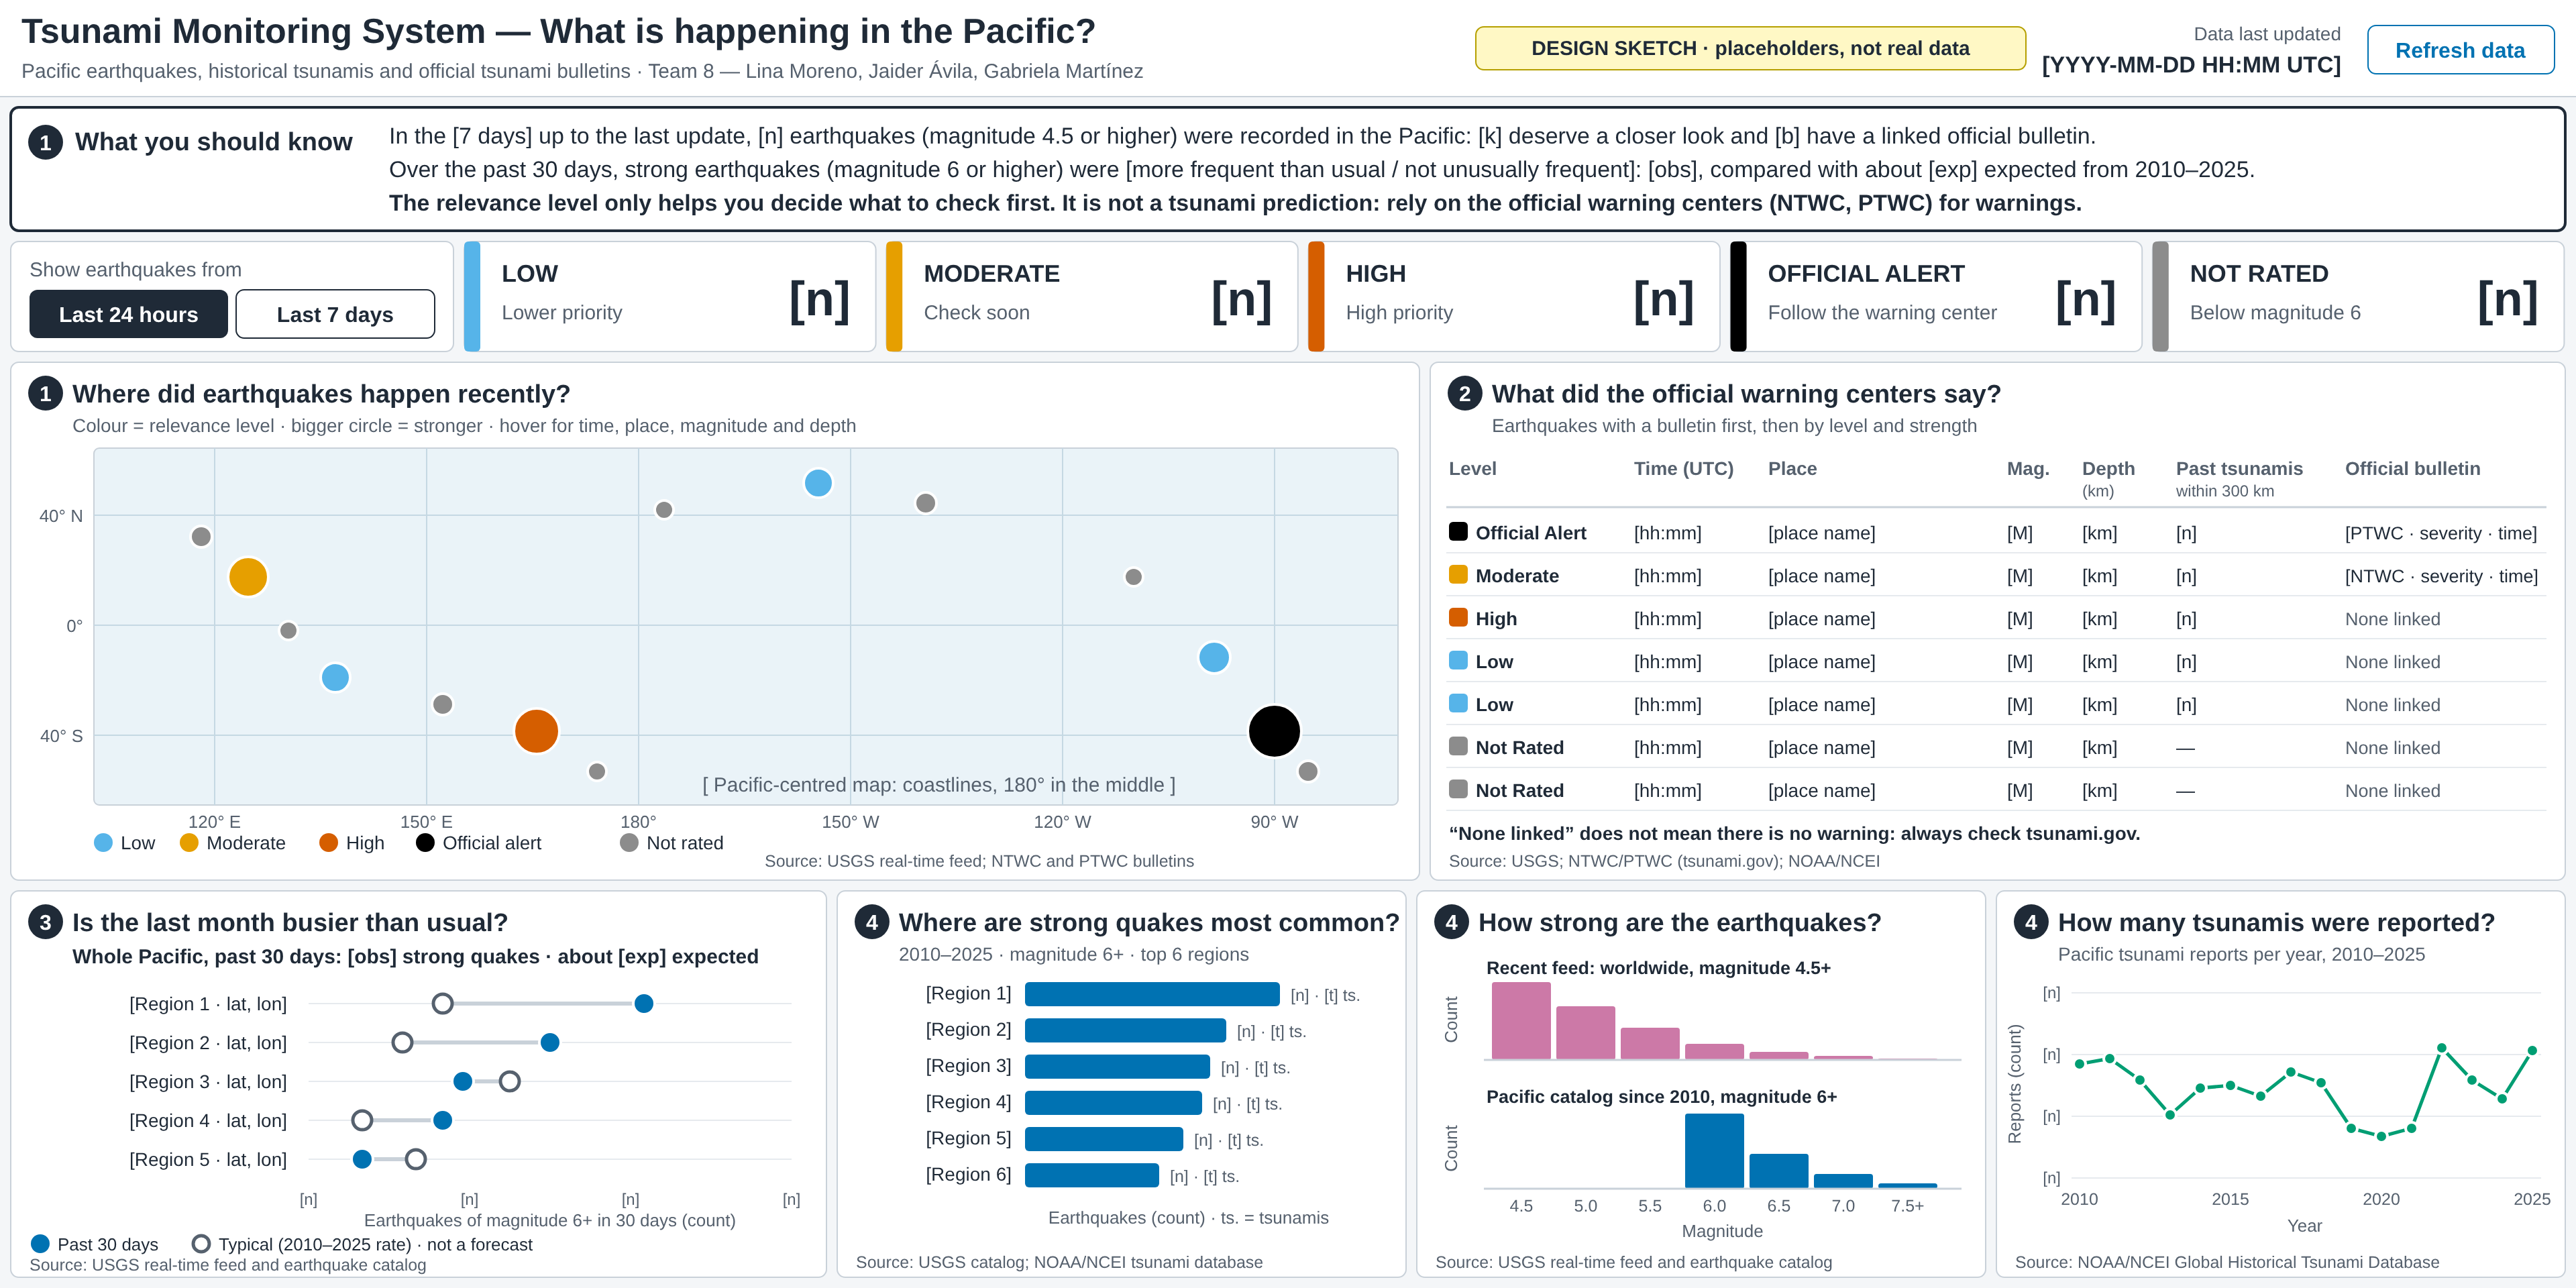
\includegraphics[width=\textheight]{figures/storytelling_sketch.png}
\caption[Design sketch of the storytelling dashboard]{Design sketch of the storytelling dashboard. Numbers 1--4 mark the reading order. All shapes and bracketed values are placeholders, not results.}
\label{fig:story-sketch}
\end{sidewaysfigure}

The bulletin table lists earthquakes with a linked bulletin first, then orders them by level and magnitude, seven rows per page, so that an official assessment is on the first page. The time filter sits above the elements it controls: the level cards, the map, the bulletin table and the first sentence of the main message. The lower row keeps fixed periods, which its titles and subtitles state. Both time windows end at the publication time of the Gold files shown in the header, not at the clock of the viewer, so an old data update cannot be mistaken for a quiet day.

\section{Main Message}
The card at the top gives the conclusion before the evidence, in three sentences. Bracketed values are filled from Gold:

\begin{quote}
In the [24 hours / 7 days] up to the last update, [$n$] earthquakes (magnitude 4.5 or higher) were recorded in the Pacific: [$k$] deserve a closer look and [$b$] have a linked official bulletin. Over the past 30 days, strong earthquakes (magnitude 6 or higher) were [more frequent than usual / not unusually frequent]: [$obs$], compared with about [$exp$] expected from 2010--2025. The relevance level only helps you decide what to check first. It is not a tsunami prediction: rely on the official warning centers (NTWC, PTWC) for warnings.
\end{quote}

The following rules keep the text accurate:
\begin{itemize}
\item $n$ counts the \path{recent_earthquakes} rows in the selected window. $k$ counts those rated MODERATE, HIGH or OFFICIAL ALERT. $b$ counts those with a \path{bulletin_source}. A zero is written as ``none'', and singular and plural forms follow the count.
\item $obs$ and $exp$ are \path{count} and \path{expected_count} of the \texttt{All Pacific query area} row of \path{historical_vs_current}. The phrase ``more frequent than usual'' is used only when \path{p_value} is below 0.05; otherwise the card says ``not unusually frequent''. This threshold is a wording rule for the single area-wide comparison and is not applied to the regional cells.
\item The third sentence is always shown. If the comparison rows are missing, the second sentence states that the comparison is not available in this data update.
\end{itemize}

\section{Components and User Stories}
\Cref{tab:story-components} maps each component to its Gold rows, its user story and the sentiment component of the course guide that it replaces. Titles are written as plain questions.

\begin{table}[!htbp]
\centering
\footnotesize
\begin{tabularx}{\textwidth}{@{}YL{3.9cm}L{1.1cm}L{2.5cm}@{}}
\toprule
Title on screen (chart type) & Gold metric and columns & Story & Guide component replaced \\
\midrule
\emph{What you should know} (text card) & \path{recent_earthquakes}, \path{historical_vs_current} & US1--US4 & Narrative summary card \\
Level cards: \emph{Low, Moderate, High, Official alert, Not rated} & \path{recent_earthquakes}: \path{relevance_level} & US4 & Sentiment distribution donut \\
\emph{Where did earthquakes happen recently?} (map) & \path{recent_earthquakes}: position, \path{magnitude}, \path{depth_km}, \path{event_time}, \path{relevance_level} & US1, US4 & Added (geographic analysis) \\
\emph{What did the official warning centers say?} (table) & \path{recent_earthquakes}: \path{bulletin_source}, \path{bulletin_severity}, \path{bulletin_sent_at}, \path{history_tsunamis} & US2, US4 & Added (official assessment) \\
\emph{Is the last month busier than usual?} (dot plot) & \path{historical_vs_current}: \path{count}, \path{expected_count}, \path{p_value}, \path{region_cell} & US3 & Sentiment trend line \\
\emph{Where are strong quakes most common?} (horizontal bars) & \path{regional_baseline}: \path{count}, \path{historical_tsunamis}, \path{region_cell} & US3 & Top keywords bars \\
\emph{How strong are the earthquakes?} (two histograms) & \path{earthquake_magnitude_distribution}: \path{source}, \path{bin_start}, \path{count} & US3 & Source comparison \\
\emph{How many tsunamis were reported?} (line) & \path{historical_tsunamis_by_year}: \path{year}, \path{count} (2010--2025) & US3 & Volume activity chart \\
\bottomrule
\end{tabularx}
\caption{Storytelling components, Gold rows and user stories.}
\label{tab:story-components}
\end{table}

US5 is covered here only by the data timestamp in the header. The last successful run and the watermark age of every source (US5), and the rejected records and quality indicators (US6), are shown in the health panel of the governance dashboard.

\section{Reading Limits Shown to the Analyst}
\begin{itemize}
\item \textbf{Relevance is not prediction.} The level is computed from magnitude, depth and nearby earlier tsunamis. In the Workshop~3 validation on the 2010--2025 catalog, 89.57\% of 163 tsunami-linked earthquakes were rated MODERATE or higher, so some earthquakes with a linked tsunami were rated LOW \cite{workshop3}.
\item \textbf{Not rated.} Only earthquakes with $M\geq6$ receive a level. Smaller ones appear in grey as \emph{Not rated}, which does not mean safe. Gold currently applies OFFICIAL ALERT only to rated earthquakes; a bulletin linked to a smaller one appears in the bulletin column.
\item \textbf{No linked bulletin.} Gold keeps only the latest accepted link of each earthquake, so ``None linked'' does not show that no warning exists. The table tells the analyst to check \url{https://www.tsunami.gov/}.
\item \textbf{Different coverage.} The magnitude histogram of the real-time feed includes earthquakes worldwide, while the catalog covers the Pacific query area; the chart labels say so. The regional bars count probable or definite tsunamis, and the yearly line counts every NOAA report.
\item \textbf{Descriptive comparison.} The dot plot lists the five regions with the smallest \path{p_value} among those with a recent earthquake. The expected count assumes the 2010--2025 average rate. The Poisson probability treats earthquakes as independent, which aftershock sequences are not, and the result is not a forecast.
\end{itemize}

\chapter{Visualization Design Decisions}
% DRAFT. After implementation: confirm that dashboard/theme.py uses the colours of tab:palette
% (usgs_realtime, ntwc, ptwc, the warning status and a "not rated" grey differ from its first version).
Both dashboards follow the same rules: one question per chart, a title in plain English, labelled axes with units, a legend whenever more than one series is drawn, a source note, and a fixed meaning for each colour \cite{edaguide}. The storytelling page is ordered as a narrative for an analyst. The governance page is ordered from summary to detail for the data team.

\section{Chart Types}
\begin{table}[!htbp]
\centering
\small
\begin{tabularx}{\textwidth}{@{}L{3.2cm}L{3cm}Y@{}}
\toprule
Information & Form & Reason \\
\midrule
Headline figures and level counts & Metric cards & A single number is read faster than a chart; four ordered levels do not need a donut. \\
Recent earthquakes & Pacific-centred map & Position is the main question. Centring on $180^\circ$ keeps the basin in one piece. Size shows magnitude and colour shows the level. \\
Earthquakes and bulletins & Table & It places each bulletin on the same row as its earthquake, with the inputs behind the level. \\
Past 30 days against typical & Dot plot with two marks per region & The gap between observed and expected is visible; the whole-area totals are written as text because their scale is much larger. \\
Most frequent regions, null and outlier rates & Sorted horizontal bars & Long labels stay readable and the order shows rank or severity. A dashed line marks the target. \\
Magnitudes by source & Two histograms on a shared magnitude axis & The sources have different areas, minimum magnitudes and periods (the Gold distribution of the real-time feed is worldwide), so each has its own count axis and a note states the difference. \\
Tsunami reports per year & Line with markers & Shows change over time. \\
Daily volume by source & Lines on a logarithmic axis & Sources differ by orders of magnitude; the axis states the scale. \\
Quality indicators & Table with target and status & Gives exact values, with problems listed first. \\
\bottomrule
\end{tabularx}
\caption{Chart selection.}
\label{tab:chart-types}
\end{table}

\section{Colour}
The palette is taken from the Okabe--Ito set, designed to remain distinguishable with common colour-vision deficiencies \cite{okabeito,wong2011}. The four relevance-level colours are reserved: they are not used for sources or quality status (\cref{tab:palette}). Sky blue and orange have low contrast against white, and no meaning depends on colour alone: levels are also written as text in cards, legends, table rows and hover boxes, map markers have an outline, and quality status has a symbol and a word.

\begin{table}[!htbp]
\centering
\small
\begin{tabularx}{\textwidth}{@{}L{2.6cm}Y@{}}
\toprule
Group & Colour assignment \\
\midrule
Relevance level & LOW sky blue (\texttt{\#56B4E9}); MODERATE orange (\texttt{\#E69F00}); HIGH vermillion (\texttt{\#D55E00}); OFFICIAL ALERT black (\texttt{\#000000}); not rated grey (\texttt{\#8C8C8C}). \\
Sources & USGS catalog blue (\texttt{\#0072B2}); USGS real-time reddish purple (\texttt{\#CC79A7}); NOAA green (\texttt{\#009E73}); NTWC dark gold (\texttt{\#8C6D1F}); PTWC violet (\texttt{\#5E3C99}). The last two extend the Okabe--Ito set. \\
Quality status & ok green; warning yellow (\texttt{\#F0E442}) with a dark outline; review reddish purple; expected grey. Status colours appear only in status marks, whose legend and labels name them. \\
Single-series charts & Blue for earthquake counts and green for NOAA tsunami reports, matching their sources. The comparison uses a filled blue dot (past 30 days) and a hollow grey dot (typical). \\
\bottomrule
\end{tabularx}
\caption{Colour encoding shared by both dashboards.}
\label{tab:palette}
\end{table}

\section{Layout}
Each dashboard fits a grid of $1920\times960$ pixels. The header gives the project, the topic, the team, the data timestamp and a refresh button. The most important content is at the top left. The storytelling layout is shown in \cref{fig:story-sketch}. The governance layout (\cref{fig:gov-sketch}) has three rows: four summary cards (total records, null rate, duplicate rate and schema compliance); missing values by field next to daily volume by source; and outlier rates, the quality table and a data-health panel (last successful run, watermark age, rejected records and matching coverage). Long lists are shortened or paged: the null-rate chart shows only fields with missing values, and the quality table shows seven rows per page.

\begin{sidewaysfigure}
\centering
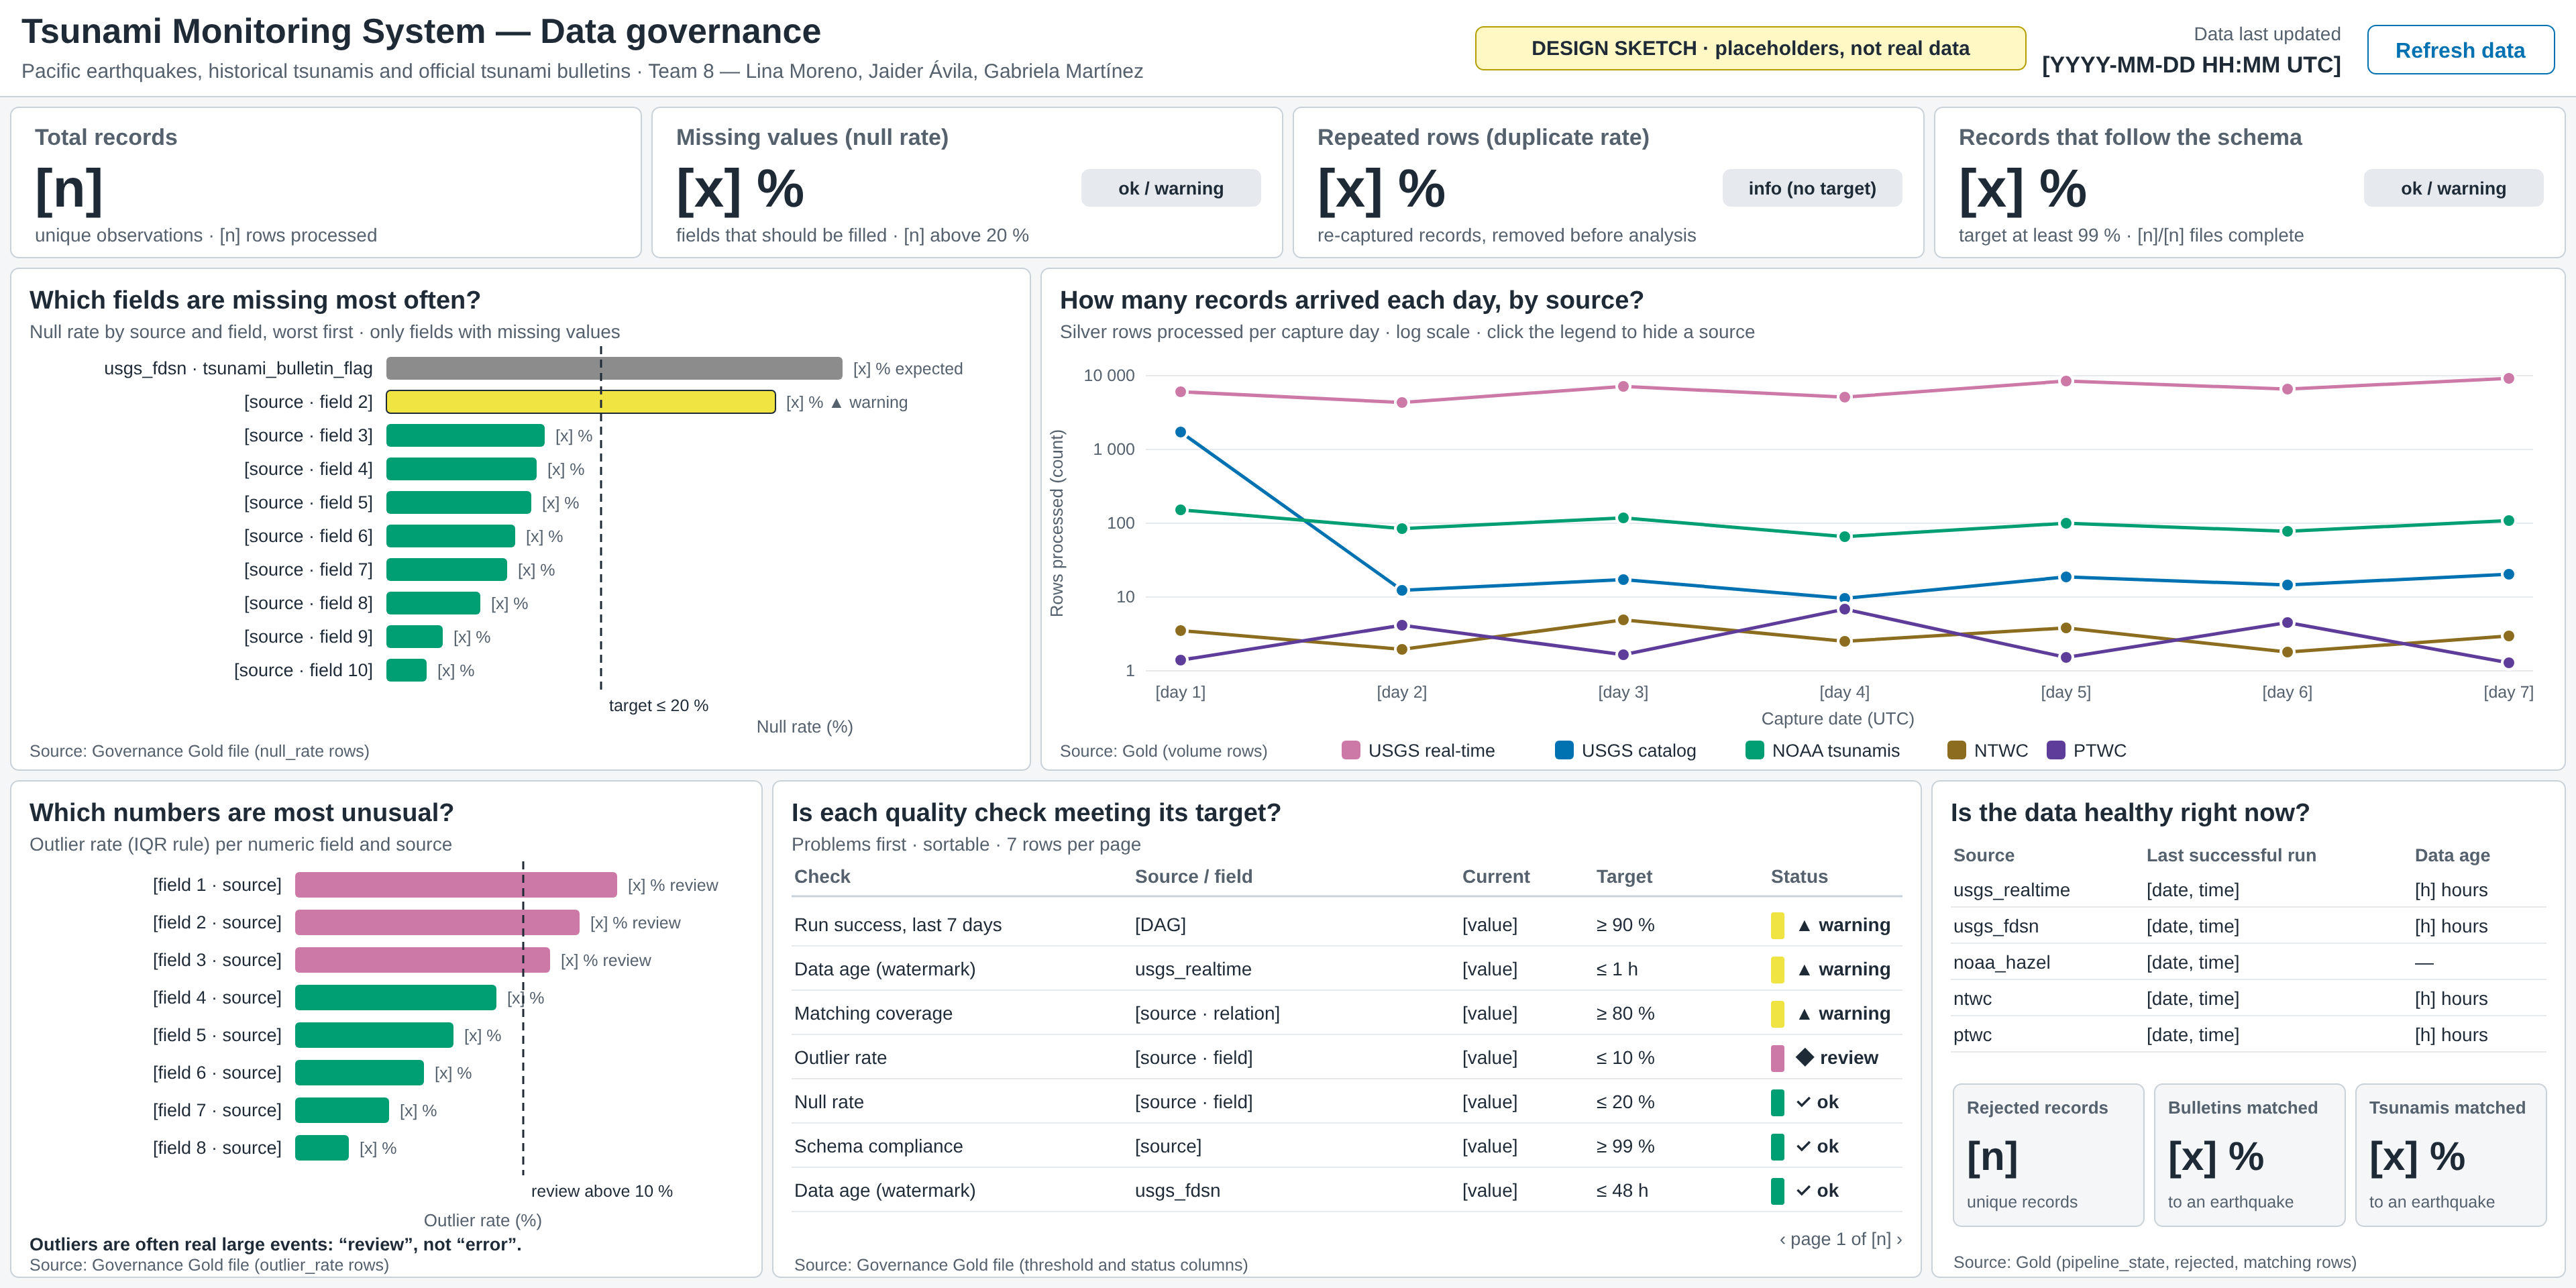
\includegraphics[width=\textheight]{figures/governance_sketch.png}
\caption[Design sketch of the governance dashboard]{Design sketch of the governance dashboard. Targets are those of \path{config/sources.yaml}; all other values, bar lengths, lines and status assignments are placeholders, not results.}
\label{fig:gov-sketch}
\end{sidewaysfigure}

\section{Labels and Context}
The storytelling page avoids pipeline terms such as Gold, watermark or null; it speaks of the last update, earthquakes and official bulletins. The governance page keeps the technical terms and states the rule behind them. Notes prevent two predictable misreadings: repeated rows are mostly records captured again from the feeds and removed before analysis, so the duplicate rate has no target; and outliers are marked for review because many are real large events. Fields that are missing by design are marked \texttt{expected}. Times are shown in UTC.

\chapter{Reproducibility Evidence}
% Guide: screenshots of the full pipeline in Airflow and both dashboards in a browser.
\textit{To be written.}

\chapter{Challenges and Resolutions}
\textit{To be written.}

\chapter{Conclusions}
% TODO: conclusions and what remains for the final project.
\textit{To be written.}

    % -------------------------------------------------------------------
    % References
    % -------------------------------------------------------------------
\begin{thebibliography}{99}
\small
\raggedright
\setlength{\bibsep}{2pt}
\bibitem{hazel} National Geophysical Data Center / World Data Service. \emph{NCEI/WDS Global Historical Tsunami Database}. NOAA National Centers for Environmental Information. doi:10.7289/V5PN93H7. Accessed through the HazEL API, \url{https://www.ngdc.noaa.gov/hazel/view/swagger}, 8 November 2026.
\bibitem{usgsfdsn} U.S.\ Geological Survey. \emph{API Documentation -- Earthquake Catalog}. \url{https://earthquake.usgs.gov/fdsnws/event/1/}. Accessed 8 November 2026.
\bibitem{usgscredit} U.S.\ Geological Survey. \emph{Acknowledging or Crediting USGS}. \url{https://www.usgs.gov/information-policies-and-instructions/acknowledging-or-crediting-usgs}. Accessed 8 November 2026.
\bibitem{usgsfeed} U.S.\ Geological Survey. \emph{Real-time Notifications, Feeds, and Web Services (GeoJSON summary feed)}. \url{https://earthquake.usgs.gov/earthquakes/feed/v1.0/geojson.php}. Accessed 7 and 9 November 2026.
\bibitem{hazelforms} NOAA National Centers for Environmental Information. \emph{HazEL tsunami event search} and \emph{earthquake search} forms. \url{https://www.ngdc.noaa.gov/hazel/view/hazards/tsunami/event-search} and \url{https://www.ngdc.noaa.gov/hazel/view/hazards/earthquake/search}. Accessed 16 November 2026.
\bibitem{tsunamigov} NOAA National Weather Service, Tsunami Warning Centers. \emph{Tsunami event feeds}. \url{https://www.tsunami.gov/}. Accessed 7 and 9 November 2026.
\bibitem{marineregions}
Flanders Marine Institute (2021).
\emph{Global Oceans and Seas, version 1}.
Marine Regions.
\url{https://doi.org/10.14284/542}.
Licensed under CC BY 4.0.
Accessed 16 November 2026.

\bibitem{taupo}
Smithsonian Institution, Global Volcanism Program (2022).
\emph{Report on Taupo (New Zealand),
30 November--6 December 2022}.
\url{https://volcano.si.edu/showreport.cfm?gvpvar=GVP.WVAR20221130-241070}.

\bibitem{tracy}
Shugar, D. H., et al.\ (2026).
\emph{A 481 m-high landslide-tsunami in a
cruise ship--frequented Alaska fjord}.
\textit{Science}. doi:10.1126/science.aec3187.
\url{https://doi.org/10.1126/science.aec3187}.
Accessed 16 November 2026.
\bibitem{workshop1} Team 8. \emph{Tsunami Monitoring System -- Workshop No.~1: Hazard Definition, Source Validation, and Data Contract}. Universidad Distrital Francisco Jos\'e de Caldas, 2026. \url{https://github.com/g8martinezsilva/tsunami-monitoring/tree/workshop-1}.
\bibitem{airflow} The Apache Software Foundation. \emph{Apache Airflow 2.10 documentation}. \url{https://airflow.apache.org/docs/apache-airflow/2.10.4/}. Accessed 17 November 2026.
\bibitem{compose} Docker Inc. \emph{Docker Compose documentation}. \url{https://docs.docker.com/compose/}. Accessed 17 November 2026.
\bibitem{postgis} PostGIS Project Steering Committee. \emph{PostGIS documentation}. \url{https://postgis.net/documentation/}. Accessed 17 November 2026.
\bibitem{pandas} The pandas development team. \emph{pandas documentation}. \url{https://pandas.pydata.org/docs/}. Accessed 17 November 2026.
\bibitem{parquet} The Apache Software Foundation. \emph{Apache Parquet documentation}. \url{https://parquet.apache.org/docs/}. Accessed 17 November 2026.
\bibitem{workshop2} Team 8. \emph{Tsunami Monitoring System -- Workshop No.~2: Technical Architecture, Historical Ingestion and Bronze/Silver Pipeline}. Universidad Distrital Francisco Jos\'e de Caldas, 2026. \url{https://github.com/g8martinezsilva/tsunami-monitoring/tree/workshop-2}.
\bibitem{pyspark} The Apache Software Foundation. \emph{PySpark documentation}. \url{https://spark.apache.org/docs/latest/api/python/}. Accessed 17 November 2026.

\bibitem{courseproject} Sierra, C. A. \emph{Course Project Description: Natural Hazard Monitoring Systems}. Data Analysis Programming, Semester 2026-II. Universidad Distrital Francisco Jos\'e de Caldas. Course handout.
\bibitem{teamassignment} Sierra, C. A. \emph{Team Project Assignment: Natural Hazard Monitoring Systems}. Data Analysis Programming, Semester 2026-II. Universidad Distrital Francisco Jos\'e de Caldas. Course handout.
\bibitem{goldguide} Sierra, C. A. \emph{Workshop No.~3: Silver-to-Gold Pipeline, Governance KPIs, and Storytelling Definition}. Data Analysis Programming, Semester 2026-I. Universidad Distrital Francisco Jos\'e de Caldas. Course handout.
\bibitem{edaguide} Sierra, C. A. \emph{Data Engineering and Visualization: ETLs, EDAs, Data Curation, and Visual Storytelling}. Semester 2026-I. Universidad Distrital Francisco Jos\'e de Caldas. Course slides.
\bibitem{curationnb} Sierra, C. A. \emph{Exploratory Data Analysis (EDA) \& Data Curation} and \emph{Data Visualization Gallery}. Data Analysis Programming, practical notebooks. Universidad Distrital Francisco Jos\'e de Caldas.
\bibitem{scipy} The SciPy community. \emph{SciPy documentation: statistical functions}. \url{https://docs.scipy.org/doc/scipy/reference/stats.html}.
\bibitem{seaborn} Waskom, M. \emph{seaborn: statistical data visualization}. \url{https://seaborn.pydata.org/}.
\bibitem{spark353} The Apache Software Foundation. \emph{Apache Spark 3.5.3 Documentation}. \url{https://spark.apache.org/docs/3.5.3/}.
\bibitem{postgresql} The PostgreSQL Global Development Group. \emph{PostgreSQL 16 Documentation: INSERT}. \url{https://www.postgresql.org/docs/16/sql-insert.html}.
\bibitem{postgis-distance} PostGIS Project Steering Committee. \emph{PostGIS Reference: ST\_DWithin}. \url{https://postgis.net/docs/ST_DWithin.html}.
\bibitem{workshop3} Team 8. \emph{Tsunami Monitoring System -- Workshop No.~3: Pipeline Improvements, Incremental Ingestion and Gold Layer}. Universidad Distrital Francisco Jos\'e de Caldas, 2026. \url{https://github.com/g8martinezsilva/tsunami-monitoring}.
\bibitem{dash} Plotly. \emph{Dash Python User Guide}. \url{https://dash.plotly.com/}.
\bibitem{dbc} Faculty AI. \emph{Dash Bootstrap Components documentation}. \url{https://dash-bootstrap-components.opensource.faculty.ai/}.
\bibitem{plotly} Plotly. \emph{Plotly Python Graphing Library}. \url{https://plotly.com/python/}.
\bibitem{okabeito} Okabe, M. and Ito, K. \emph{Color Universal Design (CUD): How to make figures and presentations that are friendly to colorblind people}. \url{https://jfly.uni-koeln.de/color/}. Accessed 27 November 2026.
\bibitem{wong2011} Wong, B. (2011). Points of view: Color blindness. \emph{Nature Methods}, 8, 441. \url{https://doi.org/10.1038/nmeth.1618}.
\end{thebibliography}

    % -------------------------------------------------------------------
    % Appendices
    % -------------------------------------------------------------------
    \begin{appendices}

\chapter{Running the Dashboards}
% TODO: exact commands (Compose and local), ports 8050 and 8051.
\textit{To be written.}

    \end{appendices}

\end{document}
